\documentclass[11pt]{report}
\usepackage{textcomp}

\usepackage{titlesec}
\titlespacing*{\section}
{0pt}{\baselineskip}{0em}
\titlespacing*{\subsection}
{0pt}{\baselineskip}{0em}

\usepackage{geometry}
\geometry{left=1in, right=1in, top=1in, textheight=9in}

\usepackage{enumitem}
\newlist{steps}{enumerate}{1}
\setlist[steps, 1]{wide=0pt, leftmargin=\parindent, label=Step \arabic*:}

\usepackage{fancyhdr}
\fancypagestyle{plain}{%
    \fancyhf{} % clear all header and footer fields
    \fancyfoot[C]{\sffamily\fontsize{.75em}{.75em}\selectfont\thepage} % except the center
    \renewcommand{\headrulewidth}{0pt}
    \renewcommand{\footrulewidth}{0pt}
}
\pagestyle{plain}

\usepackage{graphicx}
\graphicspath{ {./media/} }

\usepackage{setspace}
\doublespacing

\usepackage{minted}
\usepackage[dvipsnames]{xcolor}
\definecolor{LightGray}{gray}{0.9}

\usepackage{caption}

% make fancy title page
\makeatletter
\newcommand{\@labsection}{000}
\newcommand{\labsection}[1]{
    \renewcommand{\@labsection}{#1}
}

\newcommand{\@labnumber}{0}
\newcommand{\labnumber}[1]{
    \renewcommand{\@labnumber}{#1}
}

\newcommand{\@shortsubmitted}{1/1/70}
\newcommand{\shortsubmitted}[1]{
    \renewcommand{\@shortsubmitted}{#1}
}

\lfoot{\footnotesize \textit{University of Arkansas \\ EECS Department}}
\rfoot{\footnotesize \textsl{\@shortsubmitted}}

\renewcommand{\maketitle}{
    \newgeometry{left=1in, right=1in, top=1.75in, textheight=8.25in}
    \singlespacing
    \begin{center}
        {\huge \bf CSCE 22104} \\
        \vspace{2.5em}
        {\Large \bf Lab Report} \\
        \vspace{2em}
        \noindent\rule{20em}{0.4pt} \\
        \vspace{1em}
        {\Large \@author} \\
        \vspace{.75em}
        {\normalsize ID: 011019116} \\
        \vspace{.75em}
        {\normalsize Lab Section \@labsection} \\
        \vspace{.75em}
        {\normalsize Lab \@labnumber} \\
    \end{center}
    \newpage
    \restoregeometry
}

\makeatother


% TEXTWIDTH = 100
\begin{document}
\title{Lab Report 1}
\author{Brent Marcus Orlina}

\labsection{001}
\labnumber{9}

\shortsubmitted{4/16/25}

\maketitle

\section*{Introduction}
\begin{figure}[h!]
    \centering
    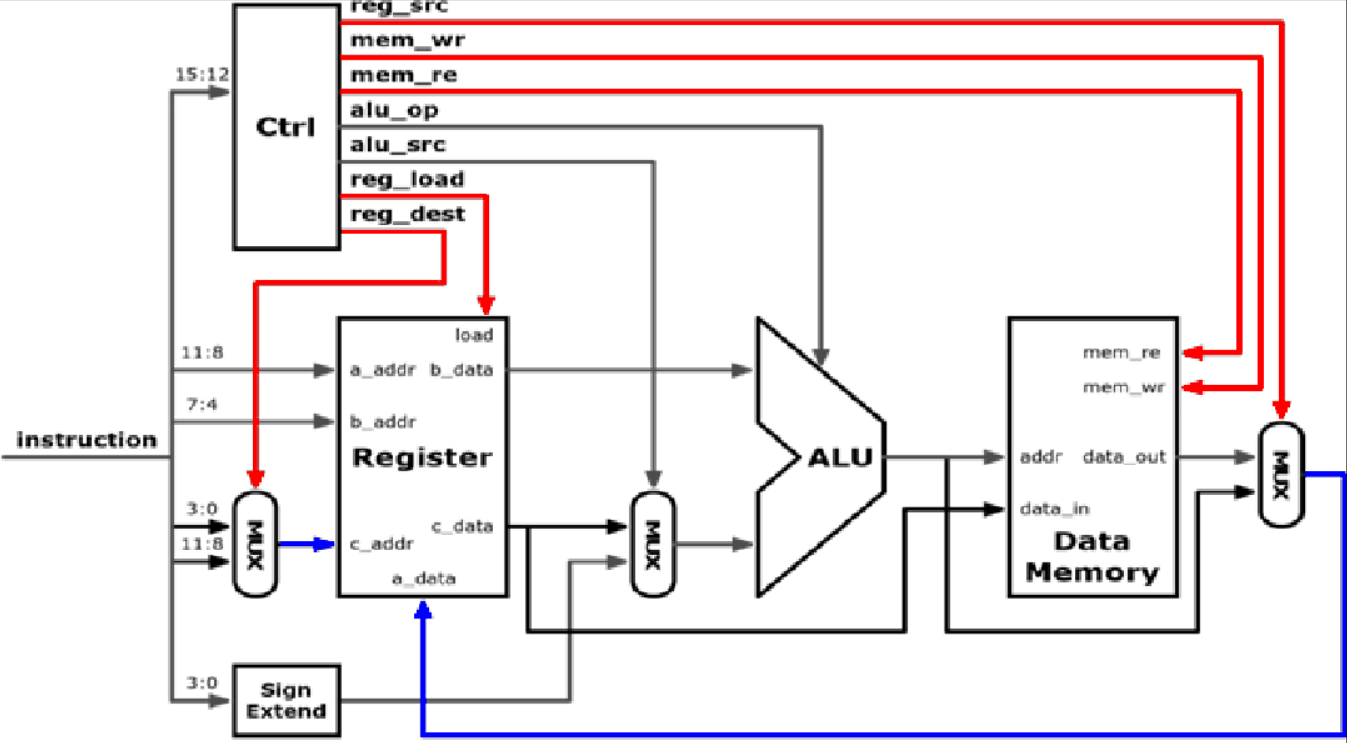
\includegraphics[width=0.95\textwidth]{circuit}
    \captionsetup{margin=0cm}
    \caption{The circuit diagram of the CPU component to be implemented.}
    \label{fig:circuit}
\end{figure}

This lab's goal was to integrate a given memory component to the CPU previously built in lab 8 to
support two additional instructions, load-word and store-word, or \verb|lw| and \verb|sw| for short
respectively, with opcodes \verb|1000| and \verb|1100|. The CPU along with any other component
within the CPU should follow the circuit diagram as shown in figure \ref{fig:circuit}.

The two new instructions are an I-type instruction, meaning that it uses the last four bits as an
immediate value. The load-word instruction, \verb|lw|, reads an address in memory, and writes the
content to the RD register provided by the instruction.  The store-word instruction, \verb|sw|,
reads the content of the RD register and stores it to an address in memory. The address read in
memory is calculated by the sum of the immediate value and the content of the RS register provided
by the instruction.

\newpage

\section*{Approach}
\begin{listing}[h!]
    \inputminted[
        frame=lines,
        breaklines,
        linenos,
        tabsize=4,
        fontsize=\footnotesize,
        bgcolor=LightGray
    ]{vhdl}{./media/memory-ports.vhd}
    \caption{The memory component's ports.}
    \label{listing:memory-ports}
\end{listing}

Listing \ref{listing:memory-ports} shows the memory component's ports. Since the memory is
synchronous to the clock, it has an input port \verb|clk|. The input ports \verb|write_en| and
\verb|read_en| allows for the memory block to written to and read, respectively. The memory should
not be written to and read simulatenously, which is ensured by the control block component. The
input port \verb|addr| is the address to be written to, by the data in input port \verb|data_in|, or
read from, outputted to the output port \verb|data_out|. Finally, the input port \verb|mem_dump| is
used for debugging purposes, and is set inactive by default.

Since
the memory component was given, the implementation details won't be shown.

\begin{listing}[h!]
    \inputminted[
        frame=lines,
        breaklines,
        linenos,
        tabsize=4,
        fontsize=\footnotesize,
        bgcolor=LightGray,
    ]{vhdl}{./media/control-ports.vhd}
    \caption{The control block component's ports.}
    \label{listing:control-ports}
\end{listing}

Listing \ref{listing:control-ports} shows the new output ports added to the control block component.
The output port \verb|ctrl_reg_src| controls whether the output of the ALU or the output of the
memory read should be written back to the register file. The output port \verb|ctrl_reg_dst|
controls whether the RT or RD register should be read for the second register read. The reason this
is done is because the store-word instruction \verb|sw| uses the RD register section of the
instruction to determine what to store into the calculated memory address and thus must be read.
This is valid since the RT section of the instruction is used as an immediate value. All other
instructions only write to the RD register and does not require it to be read.

The output port \verb|ctrl_reg_write| determines whether the register file should be written to.
Previously, the register file was always written to. However, the new \verb|sw| instruction does not
write anything to the register file, only writing into the memory component. Similarly, output ports
\verb|ctrl_mem_read| and \verb|ctrl_mem_write| control whether the memory component should be read
from or be written to since not all instructions read from or write to the memory. For example, the
\verb|lw| instruction does not write to the memory, and thus must be ensured that
\verb|ctrl_mem_write| is inactive. However, the instruction does need to read from memory, and so
it must be ensured that \verb|ctrl_mem_read| is active.


\begin{listing}[h!]
    \inputminted[
        frame=lines,
        breaklines,
        linenos,
        tabsize=4,
        fontsize=\footnotesize,
        bgcolor=LightGray,
    ]{vhdl}{./media/control-implementation.vhd}
    \caption{The control block component's implementation.}
    \label{listing:control-implementation}
\end{listing}

Listing \ref{listing:control-implementation} shows the implementation for the new control block
component. The output ports \verb|ctrl_alu_op| remains the same since the opcodes for the new
instructions, \verb|lw| and \verb|sw| since their opcodes \verb|1000| and \verb|1100| have a
\verb|00| in the last two bits, which correctly uses the ALU opcode for addition. However,
\verb|ctrl_alu_src| was changed to account for the fact that in the old implementation,
\verb|ctrl_alu_src| was simply determined by \verb|op(2)|, the second bit of the opcode. This is
incompatible with \verb|lw|'s opcode since the opcode's second bit, index-0, is inactive, implying
that the last four bits of the instruction is a register address instead of an immediate value.
Therefore, a special case has to be made for the \verb|lw| instruction to use an immediate value.

The signal \verb|ctrl_reg_src| is inactive for the \verb|lw| instruction since the data that should
be written to the register comes from the memory component, as shown in figure \ref{fig:circuit}.
Otherwise, all other instructions use the ALU's output to write to the register file, or that it
does not write to the register file at all. The signal \verb|ctrl_reg_dst| is active for the
\verb|sw| instruction since it reads from the RD register given in the instruction to provide the
data to store in the memory, as shown in figure \ref{fig:circuit}. Since instruction \verb|sw| is
the only instruction that does not write to the register file, \verb|ctrl_reg_write| is inactive for
\verb|sw| and active for all other instructions.

The signal \verb|ctrl_mem_read| is only active for instruction \verb|lw| instruction since \verb|lw|
is the only instruction that should read from the memory. Similarly, signal \verb|ctrl_mem_write| is
only active for \verb|sw| since it is the only instruction that should write to the memory. This
implementation ensures that the CPU cannot read and write to the memory simulatenously.

\begin{listing}[h!]
    \inputminted[
        frame=lines,
        breaklines,
        linenos,
        tabsize=4,
        fontsize=\footnotesize,
        bgcolor=LightGray,
    ]{vhdl}{./media/CPU-signals.vhd}
    \caption{The new signals used in the CPU implementation.}
    \label{listing:CPU-signals}
\end{listing}

Listing \ref{listing:CPU-signals} show the new signals used in the CPU implementation to support the
two new instructions. Signals \verb|RegisterSource|, \verb|RegisterDestination|,
\verb|RegisterWrite|, \verb|MemoryRead|, and \verb|MemoryWrite| are signals simply connected to the
output ports of the control block component. Since it is not especially important, this is shown in
listing \ref{listing:CPU-control} in the appendix. Signal \verb|Register2Address| is the address of
the second register chosen to be read between RD or RT, determined by the signal
\verb|RegisterDestination|. The data is outputted to the signal \verb|Register2Data| which was
formerly named \verb|RTData| since the second register that was read was always register RT.

The signal \verb|MemoryOutput| is the output of the memory component when it is read from. The
signal \verb|WriteBack| is the data to be sent back to the register file to either be written or
ignored, chosen between \verb|ALUOutput| (formerly named \verb|ALUSout|) and \verb|MemoryOutput|,
and determined by \verb|RegisterSource|.

\begin{listing}[h!]
    \inputminted[
        frame=lines,
        breaklines,
        linenos,
        tabsize=4,
        fontsize=\footnotesize,
        bgcolor=LightGray,
    ]{vhdl}{./media/CPU-decode.vhd}
    \caption{The decode and writeback phase of the CPU implementation.}
    \label{listing:CPU-decode}
\end{listing}

Listing \ref{listing:CPU-decode} shows the decode adn writeback phase of the CPU implementation. The
signal \verb|Register2Address| is set to either be register RD or RT, determined by the
\verb|RegisterDestination| signal and is connected to the input port \verb|c_addr|. The signal
\verb|RegisterWrite| is now connected to the input port \verb|load| of the register file, where it
previously was set to be constantly active. The signal \verb|Regsiter2Data| is connected to the
output port \verb|c_data|. Then, the signal \verb|ALUInput| is set to either be an immediate or the
content of the register chosen by \verb|Register2Address|, determined by the signal
\verb|ALUSource|. Finally, the signal \verb|WriteBack| is the data to be written back to the
register file, either the ALU result in the signal \verb|ALUOutput| or the data read in the memory
in the signal \verb|MemoryOutput|, determined by the \verb|RegisterSource| signal. The signal
\verb|ALUOutput| is calculated in the execute phase of the CPU, which is unchanged. Finally, the
signal \verb|MemoryOutput| is determined in the memory phase of the CPU as shown in listing
\ref{listing:CPU-memory}.

\begin{listing}[h!]
    \inputminted[
        frame=lines,
        breaklines,
        linenos,
        tabsize=4,
        fontsize=\footnotesize,
        bgcolor=LightGray,
    ]{vhdl}{./media/CPU-memory.vhd}
    \caption{The memory phase of the CPU implementation.}
    \label{listing:CPU-memory}
\end{listing}

Listing \ref{listing:CPU-memory} shows the memory phase of the CPU implementation. Its
implementation is straightforward, simply connecting the clock and the signals from the control block
component, \verb|MemoryRead| and \verb|MemoryWrite|. The address, in the input port \verb|addr|,
comes from the output of the ALU, coming from the signal \verb|ALUOutput|. The data that is written
to the memory for the \verb|sw| instruction comes from the signal \verb|Register2Data|, which is
connected to the output port \verb|c_data| of the register file. The data read at the given address
is outputted to the signal \verb|MemoryOutput|, which is used in the \verb|WriteBack| signal as
shown in \ref{listing:CPU-decode}. The debug input port \verb|mem_dump| is set to be constantly
inactive. With the memory component implemented, the CPU is completed, supporting the two new
instructions, \verb|lw| and \verb|sw|.

\section*{Experimentation}
The components were tested by writing a testbench for the CPU component. The testbench written
tested for given instructions for the CPU and were manually verified to be correct.

\section*{Results \& Discussion}
\begin{figure}[h!]
    \centering
    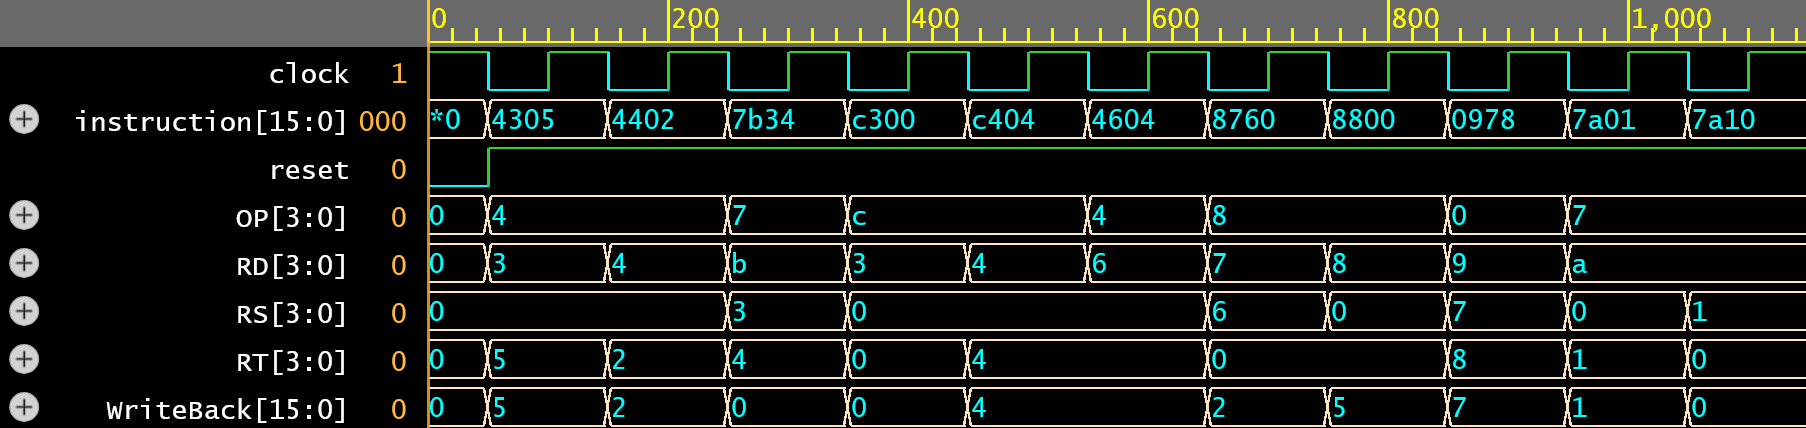
\includegraphics[width=0.95\textwidth]{CPU-waveform}
    \caption{The waveform for the CPU component.}
    \label{fig:CPU-waveform}
\end{figure}

\begin{table}[ht!]
    \centering
    \begin{tabular}{|l||c|c|c|c|c|} 
     \hline
     Instruction & op & rd & rs & rt & value (of rd) \\
     \hline
     \verb|ADDI R3, R0,  5| & \verb|0x4| & \verb|0x3| & \verb|0x0| & \verb|0x5| & \verb|5| \\ 
     \hline                                                                             
     \verb|ADDI R4, R0,  2| & \verb|0x4| & \verb|0x4| & \verb|0x0| & \verb|0x2| & \verb|2| \\
     \hline                                                                             
     %
     \verb|SW   R3,  0(R0)| & \verb|0xC| & \verb|0x3| & \verb|0x0| & \verb|0x0| & \verb|0| \\
     \hline                                                                             
     \verb|SW   R4,  4(R0)| & \verb|0xC| & \verb|0x4| & \verb|0x0| & \verb|0x4| & \verb|4| \\ 
     \hline                                                                             
     %
     \verb|ADDI R6, R0,  4| & \verb|0x6| & \verb|0x6| & \verb|0x0| & \verb|0x4| & \verb|4| \\
     \hline                                                                             
     %
     \verb|LW   R7,  0(R6)| & \verb|0x8| & \verb|0x7| & \verb|0x6| & \verb|0x0| & \verb|2| \\
     \hline                                                                             
     \verb|LW   R8,  0(R0)| & \verb|0x8| & \verb|0x8| & \verb|0x0| & \verb|0x0| & \verb|5| \\
     \hline
     %             
     \verb|ADD  R9, R7, R8| & \verb|0x0| & \verb|0x9| & \verb|0x7| & \verb|0x8| & \verb|7| \\
     \hline                                                                             
     %
    \end{tabular}
    \caption{Results of the CPU component testbench in table form.}
    \label{table:CPU-waveform_table}
\end{table}

The CPU component works as expected. Figure \ref{fig:CPU-waveform} shows the waveform of the CPU
component, correctly outputting the results of each operation. The waveform is in hex radix to
easily show the instruction in the current clock cycle and the fact that the ALU does not have any
negative results. Table \ref{table:CPU-waveform_table} shows the waveform results in table form.

\section*{Conclusions}
The memory component was integrated into the CPU correctly, shown through the testbench for the CPU.
The knowledge learned from this lab was learning how to integrate a memory component into the CPU,
along with supporting two new instructions using the memory component, correctly. This was done by
identifying what new signals are needed to allow other components to communicate with the memory
component, as well as ensuring that the right data goes to the right components under the right
instructions. 

% \newpage
% 
% \section*{References}
% \noindent
% [1]    Computer Organization 22104, EECS, University of Arkansas, “Lab 1,”  Sep. 17, 2024.
% 
% \noindent
% [2]    Computer Organization 22104, EECS, University of Arkansas, “Lab 2,”  Sep. 24, 2024.

\newpage

\section*{Appendix}
\begin{listing}[h!]
    \inputminted[
        frame=lines,
        breaklines,
        linenos,
        tabsize=4,
        fontsize=\footnotesize,
        bgcolor=LightGray,
    ]{vhdl}{./media/CPU-control.vhd}
    \caption{The CPU signals connected to the control block component.}
    \label{listing:CPU-control}
\end{listing}



% \begin{figure}[h!]
%     \centering
%     \includegraphics[width=0.9\textwidth]{foo}
%     \caption{
%         Lorem ipsum dolor sit amet, qui minim labore adipisicing minim sint cillum sint consectetur
%         cupidatat.
%     }
%     \label{fig:foo}
% \end{figure}
% 
% \newpage
% 
% \begin{figure}[h!]
%     \centering
%     \includegraphics[height=0.4\textheight]{bar}
%     \caption{Lorem ipsum something something shorter sentence}
%     \label{fig:bar}
% \end{figure}
\end{document}
